%----------------------------------------------------------------------------------------
 %	PACKAGES AND OTHER DOCUMENT CONFIGURATIONS
 %----------------------------------------------------------------------------------------
 
 % \documentclass[twoside,twocolumn]{article}
 \documentclass[oneside,onecolumn]{article}
 \usepackage{ctex}
 \usepackage{blindtext} % Package to generate dummy text throughout this template 
 
 \usepackage{amsmath,amsthm,amsfonts,amssymb,bm}
 \usepackage{mathptmx}
 
 %%\usepackage[sc]{mathpazo} % Use the Palatino font
 \usepackage[T1]{fontenc} % Use 8-bit encoding that has 256 glyphs
 \linespread{1.05} % Line spacing - Palatino needs more space between lines
 \usepackage{microtype} % Slightly tweak font spacing for aesthetics
 
 \usepackage[english]{babel} % Language hyphenation and typographical rules
 
 \usepackage[hmarginratio=1:1,columnsep=20pt]{geometry} % Document margins
 \geometry{a4paper,scale=0.8}
 \usepackage[small,labelfont=bf,up,textfont=it,up]{caption} % Custom captions under/above floats in tables or figures
 \usepackage{booktabs} % Horizontal rules in tables
 
 \usepackage{lettrine} % The lettrine is the first enlarged letter at the beginning of the text
 
 \usepackage{enumitem} % Customized lists
 \setlist[itemize]{noitemsep} % Make itemize lists more compact
 
 \usepackage{abstract} % Allows abstract customization
 \renewcommand{\abstractnamefont}{\normalfont\bfseries} % Set the "Abstract" text to bold
 \renewcommand{\abstracttextfont}{\normalfont\small\itshape} % Set the abstract itself to small italic text
 
 \usepackage{titlesec} % Allows customization of titles
 \renewcommand\thesection{\arabic{section}} % arabic numerals for the sections
 \renewcommand{\thesubsection}{\thesection.\arabic{subsection}}
 
 \titleformat{\section}[block]{\large\scshape\centering}{\thesection.}{1em}{} % Change the look of the section titles
 % \titleformat{\subsection}[block]{\large}{\thesubsection.}{1em}{} % Change the look of the section titles
 \titleformat{\subsection}[block]{\large\scshape}{\thesubsection.}{1em}{} % Change the look of the section titles
 
 \usepackage{fancyhdr} % Headers and footers
 \pagestyle{fancy} % All pages have headers and footers
 \fancyhf{} % Clear default header and footer
 \fancyfoot[C]{\thepage} % Add page number to the center of the footer
 \renewcommand{\headrulewidth}{0pt}
 
 \usepackage{titling} % Customizing the title section
 \date{}
 
 \usepackage[svgnames]{xcolor} % added by Wenyin for color
 % \usepackage{hyperref} % For hyperlinks in the PDF
 \usepackage[colorlinks=true,linkcolor=Maroon,anchorcolor=blue,citecolor=RoyalBlue,filecolor=blue,menucolor=blue,runcolor=blue,urlcolor=DodgerBlue]{hyperref} % For hyperlinks in the PDF
 
 % for multiple references with dash
 \usepackage[noadjust]{cite}
 \renewcommand{\citedash}{--}    % when \usepackage{cite}
 
 \usepackage{graphicx}
 \usepackage[export]{adjustbox}
 \graphicspath{ {./images/} }
 
 \usepackage{amsmath}
 \usepackage{amsfonts}
 \usepackage{amssymb}
 \usepackage{mathrsfs} % for \mathscr
 \usepackage{booktabs}
 \usepackage{multirow}
 
 \usepackage[T1]{fontenc}
 % To use \mdutchcal{ } as \mathcal of package dutchcal, the following commands are needed, from https://imathworks.com/tex/tex-latex-new-locally-defined-mathcal-font-for-math-equations/
 % Based on the code from mathalpha.sty: 
 \DeclareFontFamily{U}{dutchcal}{\skewchar \font =45}
 \DeclareFontShape{U}{dutchcal}{m}{n}{
 	<-> dutchcal-r}{}
 \DeclareFontShape{U}{dutchcal}{b}{n}{
 	<-> dutchcal-b}{}
 \DeclareMathAlphabet{\mdutchcal}{U}{dutchcal}{m}{n}
 \SetMathAlphabet{\mdutchcal}{bold}{U}{dutchcal}{b}{n}
 \DeclareMathAlphabet{\mdutchbcal} {U}{dutchcal}{b}{n}
 
 % \usepackage{unicode-math} % for bold math font
 % \setmathfont{XITS Math}
 
 % vector, matrix and tensor
 % \newcommand{\vect}[1]{\boldsymbol{#1}}
 % \newcommand{\vect}{\symbf}
 % \newcommand{\vect}{\mathbf} % works for English letters but not for Greek letters 
 \newcommand{\vect}[1]{\mathbf{\boldsymbol{#1}}} % works for both English and Greek letters, but it does not work with mathtime pro lite fonts, see https://tex.stackexchange.com/questions/3535/bold-math-automatic-choice-between-mathbf-and-boldsymbol-for-latin-and-greek 
 % \newcommand{\matr}[1]{\boldsymbol{\mathrm{#1}}} % \matrix is defined in LaTeX2e kernel
 \newcommand{\tens}[1]{\boldsymbol{\mathrm{#1}}}
 
 \usepackage{mathtools} % for $\intertext{text}$
 
 % for footnote without number, from https://tex.stackexchange.com/questions/170511/footnotes-without-numbering
 \let\svthefootnote\thefootnote
 % \textheight 1in
 \newcommand\blankfootnote[1]{%
 	\let\thefootnote\relax\footnotetext{#1}%
 	\let\thefootnote\svthefootnote%
 }
 \let\svfootnote\footnote
 \renewcommand\footnote[2][?]{%
 	\if\relax#1\relax%
 	\blankfootnote{#2}%
 	\else%
 	\if?#1\svfootnote{#2}\else\svfootnote[#1]{#2}\fi%
 	\fi
 }
 
 %----------------------------------------------------------------------------------------
 %	TITLE SECTION
 %----------------------------------------------------------------------------------------
 
 \setlength{\droptitle}{-4\baselineskip} % Move the title up
 
 \pretitle{\begin{center}\Huge\bfseries} % Article title formatting
 	\posttitle{\end{center}} % Article title closing formatting
 \title{Multiscale Chirping Modes Driven by Thermal Ions in a Plasma with Reactor-Relevant Ion Temperature}
 \author{Author1, Author2}
 \renewcommand{\maketitlehookd}{%
 	\begin{abstract}
 A thermal ion driven bursting instability with rapid frequency chirping, considered as an Alfvenic ion temperature gradient mode, has been observed in plasmas having reactor-relevant temperature in the DIII-D tokamak. The modes are excited over a wide spatial range from macroscopic device size to microturbulence size and the perturbation energy propagates across multiple spatial scales. The radial mode structure is able to expand from local to global in $\sim 0.1 \mathrm{~ms}$ and it causes magnetic topology changes in the plasma edge, which can lead to a minor disruption event. Since the mode is typically observed in the high ion temperature $\gtrsim 10 \mathrm{keV}$ and high- $\beta$ plasma regime, the manifestation of the mode in future reactors should be studied with development of mitigation strategies, if needed. This is the first observation of destabilization of the Alfven continuum caused by the compressibility of ions with reactor-relevant ion temperature.
 	\end{abstract}
 }
 
 %----------------------------------------------------------------------------------------
 
 \begin{document}
 \begin{sloppypar}
 % Print the title
 \maketitle

 A thermonuclear tokamak reactor requires ion temperatures $T_{i} \gtrsim 10 \mathrm{keV}$ to be self-sustaining, a large $\beta$ (ratio of plasma to magnetic pressure) to be economical, and avoidance of disruptions to be reliable. In this Letter, we describe an instability observed in high $T_{i}$ DIII-D plasmas that could jeopardize sustained and simultaneous achievement of these conditions. Unlike electrostatic iontemperature-gradient-driven (ITG) turbulence [1], the frequency spectrum of this instability consists of many distinct coherent peaks with toroidal mode numbers from $n=1$ to $>21$. Although similar wave number spectra were previously observed at high $T_{i}$ [2], these modes chirp rapidly in frequency and are strongly destabilized at high $\beta$, i.e., normalized $\beta_{N} \sim 2.5$. It is well known that chirping modes are driven by energetic particles via wave-particle resonant interaction [3], which could threaten good confinement of $\alpha$ particles in fusion reactors. However, the chirping mode investigated here is driven by resonant interaction with thermal ions having a reactor-relevant $T_{i}$, implying new challenges in the operation of high-temperature plasma in fusion reactors. The instability often triggers reconnection that could result in a minor disruption event and is unstable at a fraction of the $\beta$ limit set by ideal magnetohydrodynamic (MHD) theory, jeopardizing economical reactor operation. This dangerous instability has many properties of the theoretically predicted electromagnetic Alfven ITG (AITG) [4-6], and is consistent with the linear gyrokinetic instability analysis [7]. In contrast with the previous claim of the AITG in an ohmic plasma with $T_{i} \leq 0.75 \mathrm{keV}$ without detectable magnetic fluctuations $\tilde{b}$ [8], the observed mode, considered as the AITG, is multiscale, has appreciable $\tilde{b}$, and is driven by thermal ions with $T_{i}>10 \mathrm{keV}$.
 
 The experiment is conducted in a lower single null cross section, $80 \mathrm{kV}$ deuterium beam heated plasma with an injected power of $\sim 7 \mathrm{MW}$. The toroidal magnetic field strength is $2.1 \mathrm{~T}$ and the plasma current $I_{p}$ is $1.6 \mathrm{MA}$. The profile of safety factor $q$ monotonically increases from $\sim 0.7$ at the magnetic axis to $\sim 4$ near the plasma boundary. The plasma confinement is excellent and the $H_{98}$ factor is as high as $\sim 2.5$, forming a hot plasma core of $T_{i} \sim 15 \mathrm{keV}$ [9]. Bursting instabilities with rapid frequency chirping downward, measured by the $\mathrm{CO}_{2}$ interferometer, are routinely observed, as shown in Fig. 1(a). The wave propagates in the ion diamagnetic direction poloidally and co- $I_{p}$ direction toroidally. The real frequency of the mode in the plasma frame is $\sim 18 \mathrm{kHz}$, comparable to the ion diamagnetic drift frequency $\omega_{i}^{*}$ at the mode rational surface of the $q=1$. The frequency further chirps down to nearly $0 \mathrm{kHz}$, i.e., the Doppler frequency in the laboratory frame, in $<3 \mathrm{~ms}$. It is found that the excitation of chirping modes is rather sensitive to $T_{i}$. As one example, the chirping modes are barely observed in shot No. 178941 in Fig. 1(b), even though the plasma density,the equilibrium, and the neutral beam heating scenario agree well with shot No. 178943, as seen from Fig. 1(c). The major difference rests on the measured $T_{i}$, which is $\sim 30 \%$ lower for the case without the chirping modes, as shown in Fig. 1(d). Interestingly, in the low $T_{i}$ shot, a continuous oscillatory mode becomes dominant and a brief transition of the mode dynamics to frequency chirping is also seen, as indicated by the arrow in Fig. 1(b).
 
 \begin{figure}[htbp]
 	\centering
 	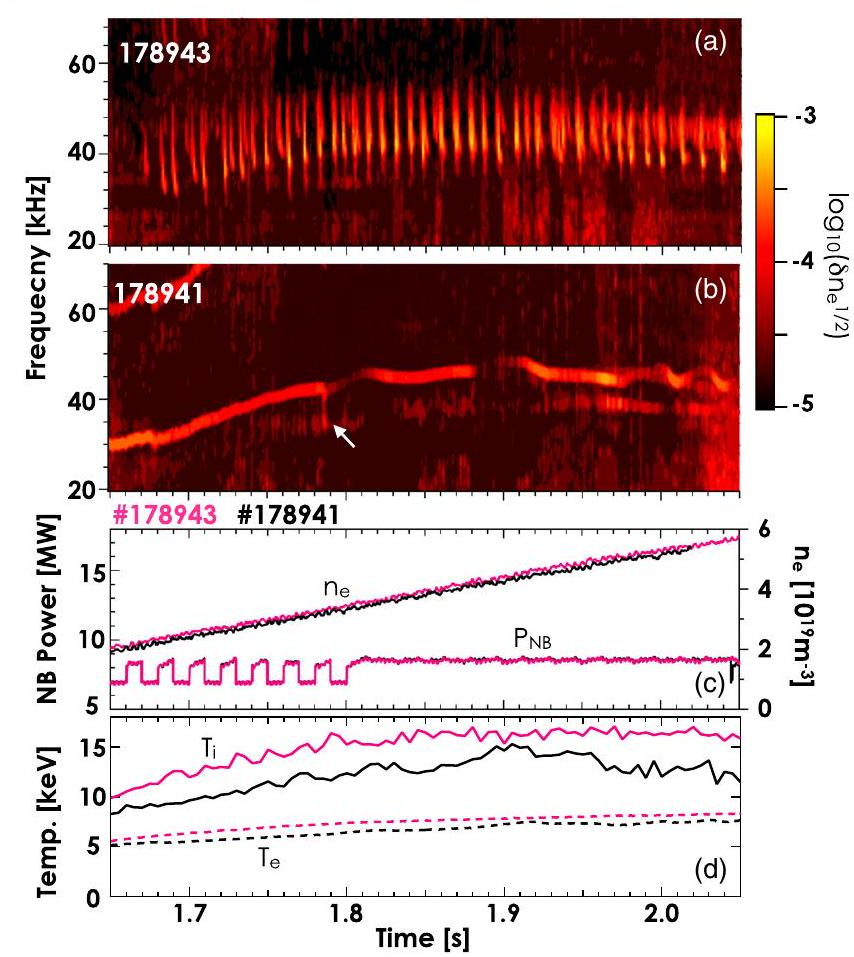
\includegraphics[max width=0.6\textwidth,max height=1.0\textheight]{2023_06_19_f8dbb752866ca158c73eg-2(1)}
 	\caption{Frequency spectra of the density fluctuations for shot No. 178943 and No. 178941 are shown in (a) and (b), respectively. The time evolutions of the line-averaged plasma density and neutral beam power in (c) and ion temperature (solid line) and electron temperature (dashed line) near the magnetic axis in (d) for shot No. 178943 (red) and No. 178941 (black).}
 	\label{figure1}
 \end{figure}
 
 
 The amplitude of the chirping modes is inversely proportional to the fast ion beta $\beta_{f}$ for the same $T_{i}$. Figure 1(a) shows that the amplitude is enhanced, as the line-averaged plasma density nearly doubles for a fixed neutral beam power between $1.8 \mathrm{~s}$ and $2.05 \mathrm{~s}$, i.e., a drop of $\beta_{f}$ by $>30 \%$ estimated by TRANSP code $[10,11]$. Statistical analysis on a database from a dedicated experiment campaign containing $>200$ chirping modes in Fig. 2(a) also shows that chirping modes with larger amplitude likely occur, when an approximation of stored fast ion energy $\left(P_{\mathrm{nb}} / n_{e}\right)$ is low and $T_{i}$ is high. Here, the variation of $P_{\mathrm{nb}} / n_{e}$ in the database mainly reflects the plasma density change, since the high $T_{i}$ is maintained by intense neutral beam power. The inverse dependence on $\beta_{f}$ is opposite to energetic particle modes, which are excited when $\beta_{f}$ exceeds a certain threshold [12].The time derivatives of the neutron flux in Fig. 2(c) across the 34 randomly sampled bursts [see Fig. 2(b)] are conditionally averaged. The result is shown as the dashed line in Fig. 2(c). The neutron rate is nearly constant across each burst. Moreover, the neutron rate predicted by the TRANSP NUBEAM code [13] using the measured plasma profiles matches the detected neutron flux well, suggesting that large loss or redistribution of the core fast ions does not occur. It should be pointed out that in this high $T_{i}$ plasma regime, TRANSP predicts the neutron yield from thermonuclear reaction is comparable to the beam-target reaction, for example $2.25 \times 10^{15} \mathrm{~N} / \mathrm{s}$ to $2 \times 10^{15} \mathrm{~N} / \mathrm{s}$ at $1.9 \mathrm{~s}$, respectively. As a result, the neutron system may not be sensitive to a modest beamtarget neutron rate change of $\leq 4 \%$ in the system detectable limit of $\sim 2 \%$, if there is any.
 \begin{figure}[htbp]
 	\centering
 	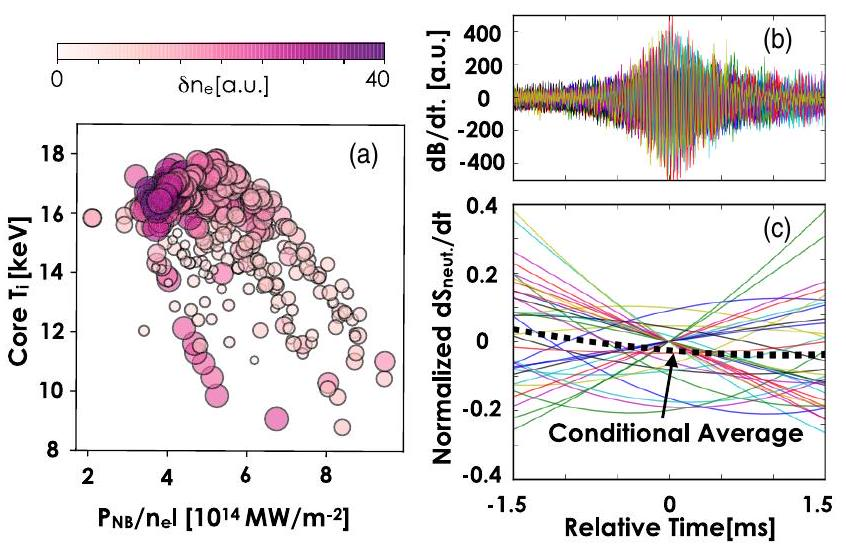
\includegraphics[max width=0.6\textwidth,max height=1.0\textheight]{2023_06_19_f8dbb752866ca158c73eg-2}
 	\caption{(a) Dependence of chirping mode amplitude on the neutral beam power normalized by the electron density $\left(\propto \beta_{f}\right)$ and the core $T_{i}$. The magnetic perturbations of 34 randomly sampled bursts (b) and corresponding time derivative of the neutron flux (c) are overlaid. The conditional averaged $d S_{\text {neut }} / d t$ is given as the dashed line in (c).}
 	\label{figure2}
 \end{figure}
 
 
 The feature of frequency chirping and amplitude bursting in a time scale of milliseconds is generally a signature of energetic particles (EP) driven instabilities. In theory, it is interpreted by a "phase locking" process that the wave frequency adapts to the resonance condition with EPs to maximize the mode drive [14]. In contrast, the data here demonstrate that bulk ions play the crucial role in the excitation of the chirping modes. Since the ion Landau damping is exponentially sensitive to $T_{i}[15]$, the strong $T_{i}$ dependence suggests that the chirping modes are excited by bulk ions and their spatial gradients.
 
 The multichannel mm-wave reflectometry diagnostic [16] and magnetic probe, which measure the local density fluctuation $\tilde{n}_{e}$ and magnetic perturbation $\tilde{b}_{\theta}$ at the plasma boundary, reveal that the chirping modes are excited over a broad range of mode frequency from $40 \mathrm{kHz}$ to $1 \mathrm{MHz}$. Magnetics data [17] show that the toroidal mode numbersof the two lowest frequency waves are 1 and 2. Since the modes appear at the $q=1$ flux surface, we infer that the poloidal and toroidal mode numbers are $(m, n)=(1,1)$ to $(21,21)$ [see Fig. 3(a)]. The estimated wavelengths of the instability span from macroscopic MHD scale down to thermal ion gyro-radii scale $\rho_{i}$, corresponding to the normalized poloidal wave number of $0.03<k_{\theta} \rho_{i}<0.6$ for the local $T_{i} \sim 12 \mathrm{keV}$. The upper bound is similar to the ITG having a typical wave number of $0.2<k_{\theta} \rho_{i}<0.5$ [18]. Interesting details of mode behaviors are summarized, as follows: (1) Right before each burst, the noticeable amplitudes of $\tilde{n}_{e}$ and $\tilde{b}_{\theta}$ in the intermediate $k_{\theta}$ range are briefly destabilized, as indicated by the arrows in Fig. 3(a) and circles in Fig. 3(b). The peak-to-peak frequency spacing in the staircase-shaped frequency spectra is $32 \mathrm{kHz}$, close to the frequency at the end of the chirping of the lowest $k_{\theta}$ wave, i.e., $31.5 \mathrm{kHz}$. This indicates that the trigger mechanism of the burst may relate to the multiscale perturbation energy transfer via resonant wave-wave coupling. (2) In the first half of the burst, which corresponds to the rapid frequency chirping period, the $\tilde{b}_{\theta}$ over a broad $k_{\theta}$ range are detected without detectable $\tilde{n}_{e}$. However, in the latter half of the bursts, which corresponds to stationary frequency period, the $\tilde{b}_{\theta}$ of the higher- $k_{\theta}$ waves suddenly reduced and the $\tilde{n}_{e}$ is significantly enhanced. The transition from the dominant $\tilde{b}_{\theta}$ to $\tilde{n}_{e}$ are indicated by the dotted lines in Fig. 3. The similar time traces of $\tilde{n}_{e}$ are observed across the burst in a broad range of minor radii and therefore it is not owing to the effect of local measurements. In addition, in rare cases, the $\tilde{b}_{\theta}$ in the high- $k_{\theta}$ range is absent.
 \begin{figure}[htbp]
 	\centering
 	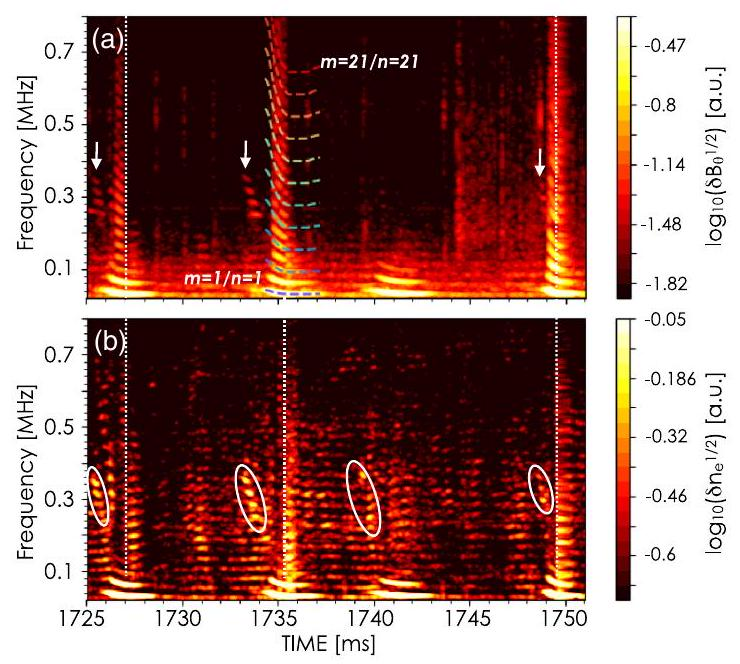
\includegraphics[max width=0.6\textwidth,max height=1.0\textheight]{2023_06_19_f8dbb752866ca158c73eg-3(1)}
 	\caption{Frequency spectra of the magnetic fluctuation at the plasma boundary (a) and density fluctuation spectra around the $q=1$ flux surface (b) in shot No. 178942 .}
 	\label{figure3}
 \end{figure}
 
 
 The observed higher- $k_{\theta}$ waves are not an artificial effect from the fast Fourier transform on a distorted waveform. The higher- $k_{\theta}$ waves are real, because the high- $k_{\theta}$ wavesexist independently from the lowest $k_{\theta}$ wave. The $\tilde{n}_{e}$ perturbations in the medium $k_{\theta}$ range are also marginally unstable between the bursts and are often stabilized right after the bursts, for example at $1728 \mathrm{~ms}$ in Fig. 3(b). According to theory, multiscale excitation of the modes could be caused by nonlinear wave-wave coupling, referred to as a pair-interaction cascade [19]. It is also possible that the nonlinear coupling is through waveparticle interaction [20]. Clarification of the nonlinear excitation mechanism needs further experimental effort and is left for future work.
 \begin{figure}[htbp]
 	\centering
 	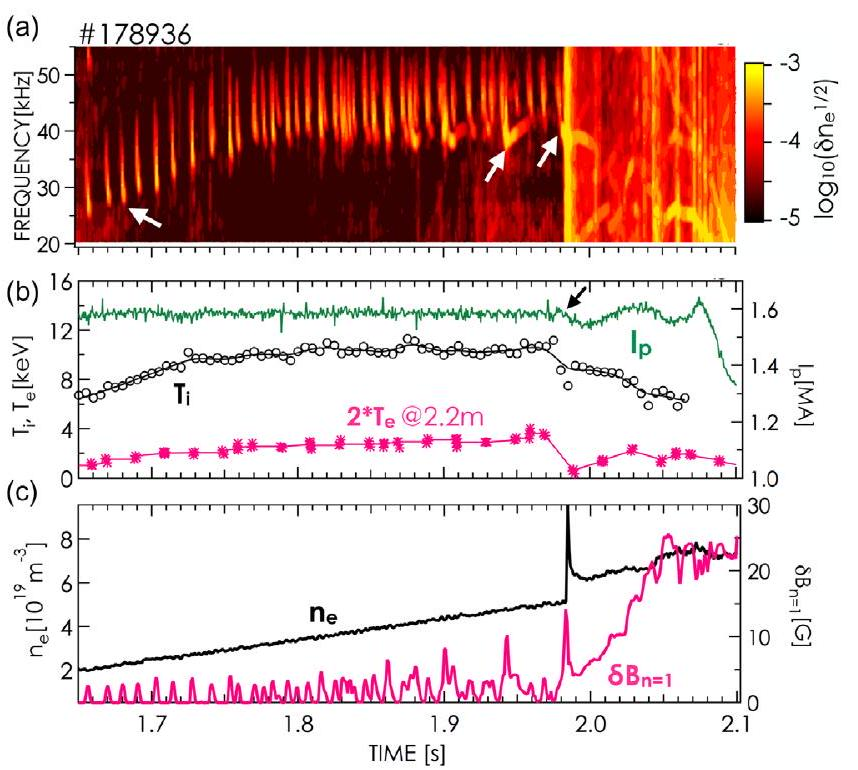
\includegraphics[max width=0.6\textwidth,max height=1.0\textheight]{2023_06_19_f8dbb752866ca158c73eg-3}
 	\caption{(a) Frequency spectra of density fluctuation measured by a $\mathrm{CO}_{2}$ interferometer. Time evolution of plasma current, ion temperature near the $q=1$ flux surface and electron temperature at $R=2.2 \mathrm{~m}$ in (b), volume-averaged electron density and integrated magnetic fluctuation of $n=1$ in (c).}
 	\label{figure4}
 \end{figure}
 
 
 The chirping modes may be benign with respect to their impact on neutron production, but lead to minor disruption events for a few times in a short dedicated experiment. Figure 4 shows that at the end of the frequency chirping of $t \sim 1.9837 \mathrm{~s}$, a moderate $I_{p}$ spike [see the arrow in Fig. 4(b)] is accompanied by a substantial density increase. The $I_{p}$ spike is an indicator of the current profile redistribution, usually characterized as a disruption event. The density spike suggests a large inward impurity flux from the first wall. Note that the plasma $\beta_{N}$ is $\sim 2.7$ at the event, well below the ideal $\beta_{N}$ limit.
 
 To understand why some chirping modes trigger minor disruption events but not others, the radial mode structures of three chirping modes, indicated by three arrows in Fig. 4(a), are compared. Figure 5 shows time evolution of electron temperature fluctuation $\tilde{T}_{e}$ profiles measured by electron cyclotron emission. The magnetic fluctuations are overlaid as a reference. At $t \sim 1.685 \mathrm{~s}$, the burst amplitude is relatively low. The observed $\tilde{T}_{e}$ localizesat the $q=1$ flux surface at $R \sim 1.9 \mathrm{~m}$ with a radial mode width of $\sim 10 \mathrm{~cm}$, as seen in Fig. 5(a). The phase difference in the radial direction is nearly zero, i.e., a kink parity persists across the entire burst.
 \begin{figure}[htbp]
 	\centering
 	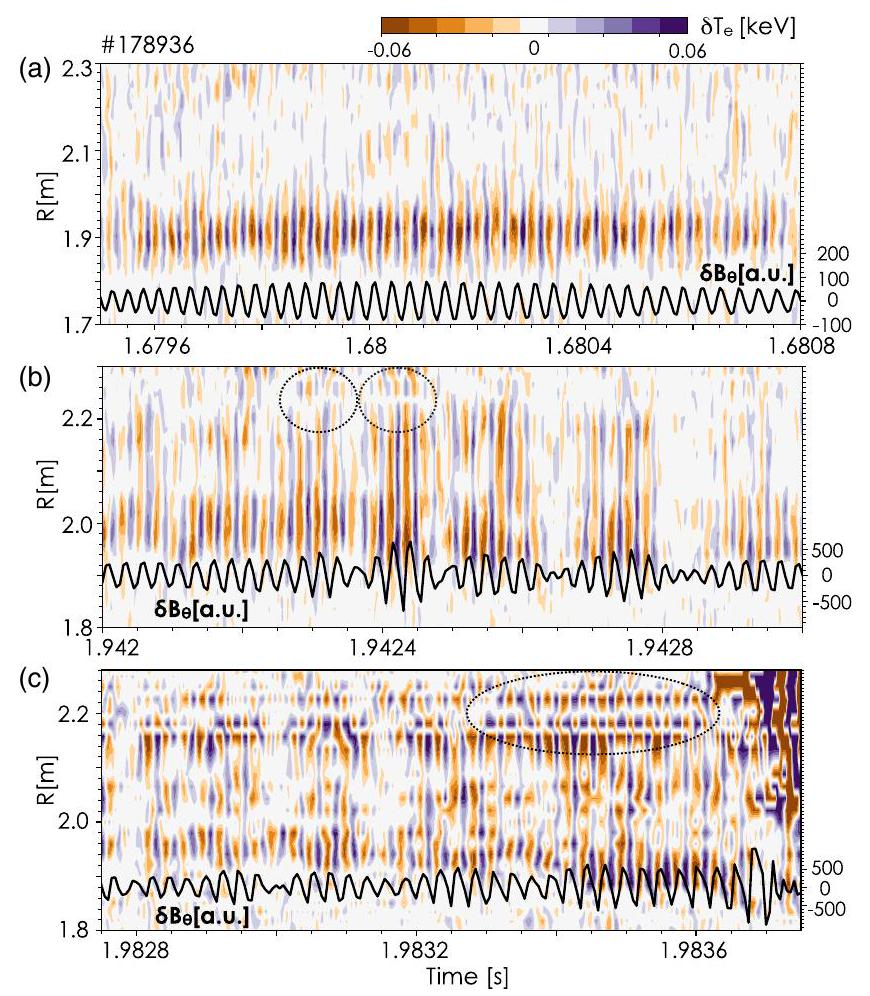
\includegraphics[max width=0.6\textwidth,max height=1.0\textheight]{2023_06_19_f8dbb752866ca158c73eg-4}
 	\caption{Time evolutions of the electron temperature fluctuations of the three chirping modes [marked by the three arrows in Fig. 4(a)] at $\sim 1.678 \mathrm{~s}, \sim 1.942 \mathrm{~s}$, and $\sim 1.983 \mathrm{~s}$ in (a)-(c), respectively. The evolution of the magnetic probe signals are overlaid together. Note that although the optical thickness outside $\sim 2.24 \mathrm{~m}$ in Fig. 3(c) is thin, synthetic electron cyclotron emission suggests that the fluctuation is dominated by the $\tilde{T}_{e}$.}
 	\label{figure5}
 \end{figure}
 
 
 As the mode amplitude substantially increases around $t \sim 1.942$ s, i.e., about $50 \mathrm{~ms}$ before the minor disruption, the mode structure noticeably changes in the following ways: (1) It shifts radially outward by $\sim 5 \mathrm{~cm}$, tracking the outward radial shift of the $q=1$ flux surface. (2) The modes transiently expand in the radial direction, covering a broad radial range from the plasma core of $1.95 \mathrm{~m}$ to the edge of $2.28 \mathrm{~m}$. Note that the expansion occurs in a short time scale of $\sim 0.1 \mathrm{~ms}$, accompanied by a rapid, appreciable increase of magnetic perturbation. (3) As the mode expands, the kink parity is only preserved in the plasma core. A radial $\pi$-phase jump, i.e., tearing parity, is observed across the $R=2.22 \mathrm{~m}$ [see the circles in Fig. 5(b)]. It is a sign of forced magnetic reconnection, which leads to a magnetic topology change to islandtype in the plasma edge. As the mode amplitude rapidly decays, the $\pi$-phase jump cannot be sustained and promptly disappears. A more systematic magnetic topology change occurs and lasts for $\sim 0.5 \mathrm{~ms}$ right before the minor disruption. As seen from the circle in Fig. 5(c), multiple $\pi$-phase jumps are found at $R=2.17 \mathrm{~m}, 2.2 \mathrm{~m}$, and $2.24 \mathrm{~m}$. According to the equilibrium reconstructed by the EFIT code [21], these radial locations are well aligned with the major rational surfaces of $q=2, q=3$ and $q=4$, respectively. The chirping mode generates multihelicity island chains at the plasma edge in a time scale of submilliseconds. Later, the $T_{e}$ at $R=2.2 \mathrm{~m}$, measured by the Thomson scattering system, suddenly decreases from $1.9 \mathrm{keV}$ to $0.25 \mathrm{keV}$, as shown in Fig. 4(b). The reduction can be attributed to the overlap of multihelicity island chains, which leads to a stochastic plasma boundary $[22,23]$. However, it should be emphasized that the physics is distinct from the disruptions induced by neoclassical tearing modes (NTMs). The growth time of a NTM from a pre-existing small magnetic islands, takes tens of milliseconds, i.e., significantly longer by three orders of magnitude. The observed magnetic reconnection is speculated to be driven directly by Alfvenic fluctuation, similar to those reported in simulation [24]. Arguably, this is much more dangerous for plasma operation, due to the extremely short time scale for actuators to respond.
 
 The observed rapid broadening and shrinkage of the mode structure in a time scale of submilliseconds differs from the picture of MHD theory. In gyrokinetic theory, EP or thermal ions cause rapid changes in the eigenfunction. That is, the mode structure is partly determined by the source of free energy via the wave-particle resonant interaction, referred to as the nonperturbative feature [25]. Therefore, the resonance condition between the chirping modes and thermal ions is studied. For passing particles, the resonance condition in a tokamak is given by $f_{m}-l f_{\mathrm{tr}, p}+n f_{\mathrm{tr}, t}=0$, where $f_{m}$ is the mode frequency, $n$ is the toroidal mode number, $l$ is an arbitrary integer, and $f_{\mathrm{tr}, p}$ and $f_{\mathrm{tr}, t}$ are poloidal and toroidal transit frequencies, calculated by the orbit following code (ASCOT5) [26]. Using $f_{m}=18 \mathrm{kHz}$ and $n=1$, the resonance lines in energy- $R$ space are estimated for deuterium ions of pitch $v_{\|} / v=0.7,0.8$, and 0.9 , as shown in Fig. 6. The carbon temperature from charge exchange recombination spectroscopy is overlaid and the shaded band indicates the high-energy tail of the bulk ions, up to $1.9 T_{i}$. It is found that, due to the high $T_{i}$, the fundamental resonance of $l=-1$ is predominantly satisfied in the phase space of the thermal ion tail over nearly the entire minor radius.
 
 Using the experiment data, linear analysis solving electromagnetic gyrokinetic equations (CGYRO code) [7] find that the most unstable modes at the $q=1$ flux surface at $1800 \mathrm{~ms}$ of shot No. 178936 are low- $n$ kinetic ballooning modes (KBM) or AITG [see the red curve in Fig. 6(b)], which are linearly unstable over a broad rangeof $k_{\theta} \rho_{s}$. The growth rate $\gamma$ is generally smaller at higher $k_{\theta} \rho_{s}$ waves, and peaks at $k_{\theta} \rho_{s} \sim 0.09$, i.e., $k_{\theta} \sim 0.25 \mathrm{~cm}^{-1}$ for $\rho_{s}=0.35 \mathrm{~cm}$, corresponding to a long wavelength perturbation, distinguished from electrostatic ITG. A scan of $T_{i}$ using the measured electron beta $\beta_{e}$ confirms that the $\gamma$ increases at higher $T_{i}$. For fixed $T_{i}$, the modes are more unstable at higher $\beta_{e}$ (data not shown here). The real frequency of the waves is $\sim 1.5$ times of the observed frequency in plasma frame. Other similarities to the theoretically predicted AITG [4-6] are discussed, as follows: (1) The mode propagates in the ion diamagnetic drift direction in the frequency near $\omega_{i}^{*}$. (2) The mode can be driven by a finite gradient of the $T_{i}$, without contribution from the EPs and the excitation requires $\nabla T_{i}$ to exceed a threshold value. (3) The plasma regime is close to, but below the ideal MHD $\beta$ limit. (4) The free energy source is from kinetic wave-particle interactions with the thermal ions, consistent with calculated resonances between the chirping modes and transit motion of the bulk ions. It is also consistent with the strong nonperturbative feature of the mode structure. (5) The $\eta_{i}$ ( $\equiv \partial \ln T_{i} / \partial \ln n_{i}$ ) exceeds the theory-predicted threshold $\eta_{i c}$ [Eq. (31) of [4]] for the onset of unstable Alfven continuum due to compressibility of core ions [4-6]. For example, using the data at $\sim 1.73 \mathrm{~s}$ in shot No. 178936 , the $\eta_{i}$ is 1.75 , larger than the estimated $\eta_{i c}$ of 1.25 for the most unstable $k$ wave of $m=8 / n=8$. The estimation also finds that the most unstable modes belong to the strongly coupled $\mathrm{KBM}$ and $\beta$-induced Alfven eigenmodes branch [4,27].
 \begin{figure}[htbp]
 	\centering
 	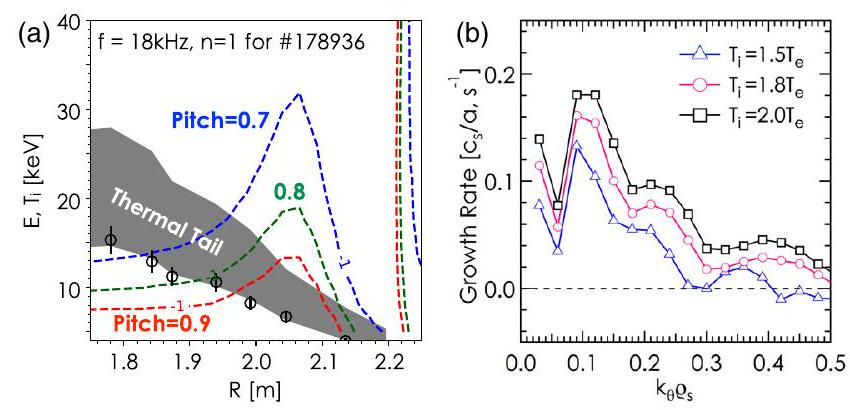
\includegraphics[max width=0.6\textwidth,max height=1.0\textheight]{2023_06_19_f8dbb752866ca158c73eg-5}
 	\caption{(a) The resonance lines in energy- $R$ space at the midplane for pitch 0.7 (blue), 0.8 (green), and 0.9 (red). The measured $T_{i}$ is represented by the circles and its high-energy thermal tail is indicated by the shaded band. (b) The growth rate (normalized by the ion sound speed, $c_{s}$ ) of AITG over a range of the $k_{\theta} \rho_{s}$ for fixed $\beta_{e}$, where $\rho_{s} \equiv\left(m_{i} T_{e}\right)^{0.5} / e B$. In experiment, $T_{i}$ is $1.8 T_{e}$ at the $q=1$ flux surface.}
 	\label{figure6}
 \end{figure}
 
 
 Since the modes become unstable at a fraction of the ideal MHD $\beta$ limit at high ion temperature, and can lead to minor disruptions through extremely rapid field line reconnection and stochastization, their manifestation in future reactors should be carefully studied with development of mitigation strategies, if necessary. 
 
 \clearpage
 \section*{References}
 [1] W. Horton, D.-I. Choi, and W. M. Tang, Phys. Fluids 23, 590 (1980).
 
 [2] R. Nazikian, H. L. Berk, R. V. Budny, K. H. Burrell, E. J. Doyle, R. J. Fonck, N. N. Gorelenkov, C. Holcomb, G. J. Kramer, R. J. Jayakumar, R. J. La Haye, G. R. McKee, M. A. Makowski, W. A. Peebles, T. L. Rhodes, W. M. Solomon, E. J. Strait, M. A. VanZeeland, and L. Zeng, Phys. Rev. Lett. 96, 105006 (2006).
 
 [3] B. N. Breizman and S. E. Sharapov, Plasma Phys. Controlled Fusion 53, 054001 (2011).
 
 [4] F. Zonca, L. Chen, and R. A. Santoro, Plasma Phys. Controlled Fusion 38, 2011 (1996).
 
 [5] F. Zonca, L. Chen, R. A. Santoro, and J. Q. Dong, Plasma Phys. Controlled Fusion 40, 2009 (1998).
 
 [6] F. Zonca, L. Chen, J. Q. Dong, and R. A. Santoroc, Phys. Plasmas 6, 1917 (1999).
 
 [7] J. Candy, E. Belli, and R. Bravenec, J. Comput. Phys. 324, 73 (2016).
 
 [8] W. Chen et al., Europhys. Lett. 116, 45003 (2016).
 
 [9] P. B. Snyder et al., Nucl. Fusion 59, 086017 (2019).
 
 [10] R. J. Hawryluk, An empirical approach to tokamak transport, in Physics of Plasmas Close to Thermonuclear Conditions, edited by B. Coppi et al. (CEC, Brussels, 1980), Vol. 1, pp. 19-46.
 
 [11] B. A. Grierson, X. Yuan, M. Gorelenkova, S. Kaye, N. C. Logan, O. Meneghini, S. R. Haskey, J. Buchanan, M. Fitzgerald, S. P. Smith et al., Fusion Sci. Technol. 74, 101 (2018).
 
 [12] L. Chen, Phys. Plasmas 1, 1519 (1994).
 
 [13] A. Pankin, D. Mccune, R. Andre, G. Bateman, and A. Kritz, Comput. Phys. Commun. 159, 157 (2004).
 
 [14] H. L. Berk, B. N. Breizman, J. Candy, M. Pekker, and N. V. Petviashvili, Phys. Plasmas 6, 3102 (1999).
 
 [15] S. D. Pinches, I. T. Chapman, Ph. W. Lauber, H. J. C. Oliver, S. E. Sharapov, K. Shinohara, and K. Tani, Phys. Plasmas 22, 021807 (2015).
 
 [16] W. A. Peebles, T. L. Rhodes, J. C. Hillesheim, L. Zeng, and C. Wannberg, Rev. Sci. Instrum. 81, 10D902 (2010).
 
 [17] J. D. King, E. J. Strait, R. L. Boivin, D. Taussig, M. G. Watkins, J. M. Hanson et al., Rev. Sci. Instrum. 85, 083503 (2014).
 
 [18] A. M. Dimits et al., Nucl. Fusion 41, 1725 (2001).
 
 [19] R. H. Kraichhan, Phys. Fluids 10, 1417 (1967).
 
 [20] F. Zonca, L. Chen, S. Briguglio, G. Fogaccia, A. V. Milovanov, Z. Qiu, G. Vlad, and X. Wang, Plasma Phys. Controlled Fusion 57, 014024 (2015).
 
 [21] L. L. Lao, J. R. Ferron, R. J. Groebner, W. Howl, H. St. John, E. J. Strait, and T. S. Taylor, Nucl. Fusion 30, 1035 $(1990)$. [22] X. D. Du, M. W. Shafer, Q. M. Hu, T. E. Evans, E. J. Strait, S. Ohdachi, and Y. Suzuki, Phys. Plasmas 26, 042505 $(2019)$
 
 [23] Q. M. Hu, X. D. Du, Q. Yu, N. C. Logan, E. Kolemen, R. Nazikian, and Z. H. Jiang, Nucl. Fusion 59, 016005 (2019).
 
 [24] A. Bierwage, K. Shinohara, Y. Todo, N. Aiba, M. Ishikawa, G. Matsunaga, M. Takechi, and M. Yagi, Nat. Commun. 9, $3282(2018)$. [25] Z. Wang, Z. Lin, I. Holod, W. W. Heidbrink, B. Tobias, M. Van Zeeland, and M. E. Austin, Phys. Rev. Lett. 111, 145003 (2013).
 
 [26] E. Hirvijoki, A. Snicker, T. Korpilo, P. Lauber, E. Poli, M. Schneller, and T. Kurki-Suonio, Comput. Phys. Commun. 183, 2589 (2012).
 
 [27] I. Chavdarovski and F. Zonca, Phys. Plasmas 21, 052506 $(2014)$
 
 	%----------------------------------------------------------------------------------------
 \end{sloppypar}	
 \end{document}
